
\section{Transit method}
\label{sec:transit}


Among all exoplanet discovery methods, the transit method has most exoplanet discoveries on its name. At the time of writing, over 75\% (3343 in total) of the known exoplanets (4424 in total) were discovered using this method\footnote{\url{https://exoplanetarchive.ipac.caltech.edu/docs/counts_detail.html}}. Of the other methods, the radial velocity method is the most successful, covering about 20\% of the exoplanet discoveries. The radial velocity method works by measuring the shifts in the spectrum of a star which are due to the gravitational pull of an orbiting planet. While this used to be the prominent method for exoplanet discovery, nowadays it is mostly used to complement the transit method as a means of confirming exoplanet candidates, or characterizing planetary systems. Anther method closely related to the transit method uses transit timing variations (TTVs) of transiting planets to infer the presence of an additional planet in the same system. TTVs are deviations from the expected periodicity of a signal, which could be caused by a disturbing planet in a different orbit around the same star. Other methods to exoplanet discovery exist, but for the purpose of this thesis we do not go into depth for these methods.

Most planets in our Solar System can be directly observed with a small telescope or even the unaided eye. For the observation of exoplanets, distances between stars plays a role, which are large compared to the distances between stars and planets. The distance between Earth and the Sun is 1 Astronomical Unit (1 AU = \num{1.496e8} km) and the distance to the nearest star is about $10^5$ AU. Exoplanets are thus far away and form a compact system together with their host star as observed from Earth. This makes direct imaging of exoplanets difficult. Therefore, most methods rely on indirect measurements of potential exoplanets. This is also the case for the transit method, for which only the brightness of a star is monitored over time. Dips in the observed brightness are used as indication of an exoplanet passing in front of the stellar disk. A requirement for this method is therefore that the system is seen edge-on. 

\begin{figure}
    \centering
    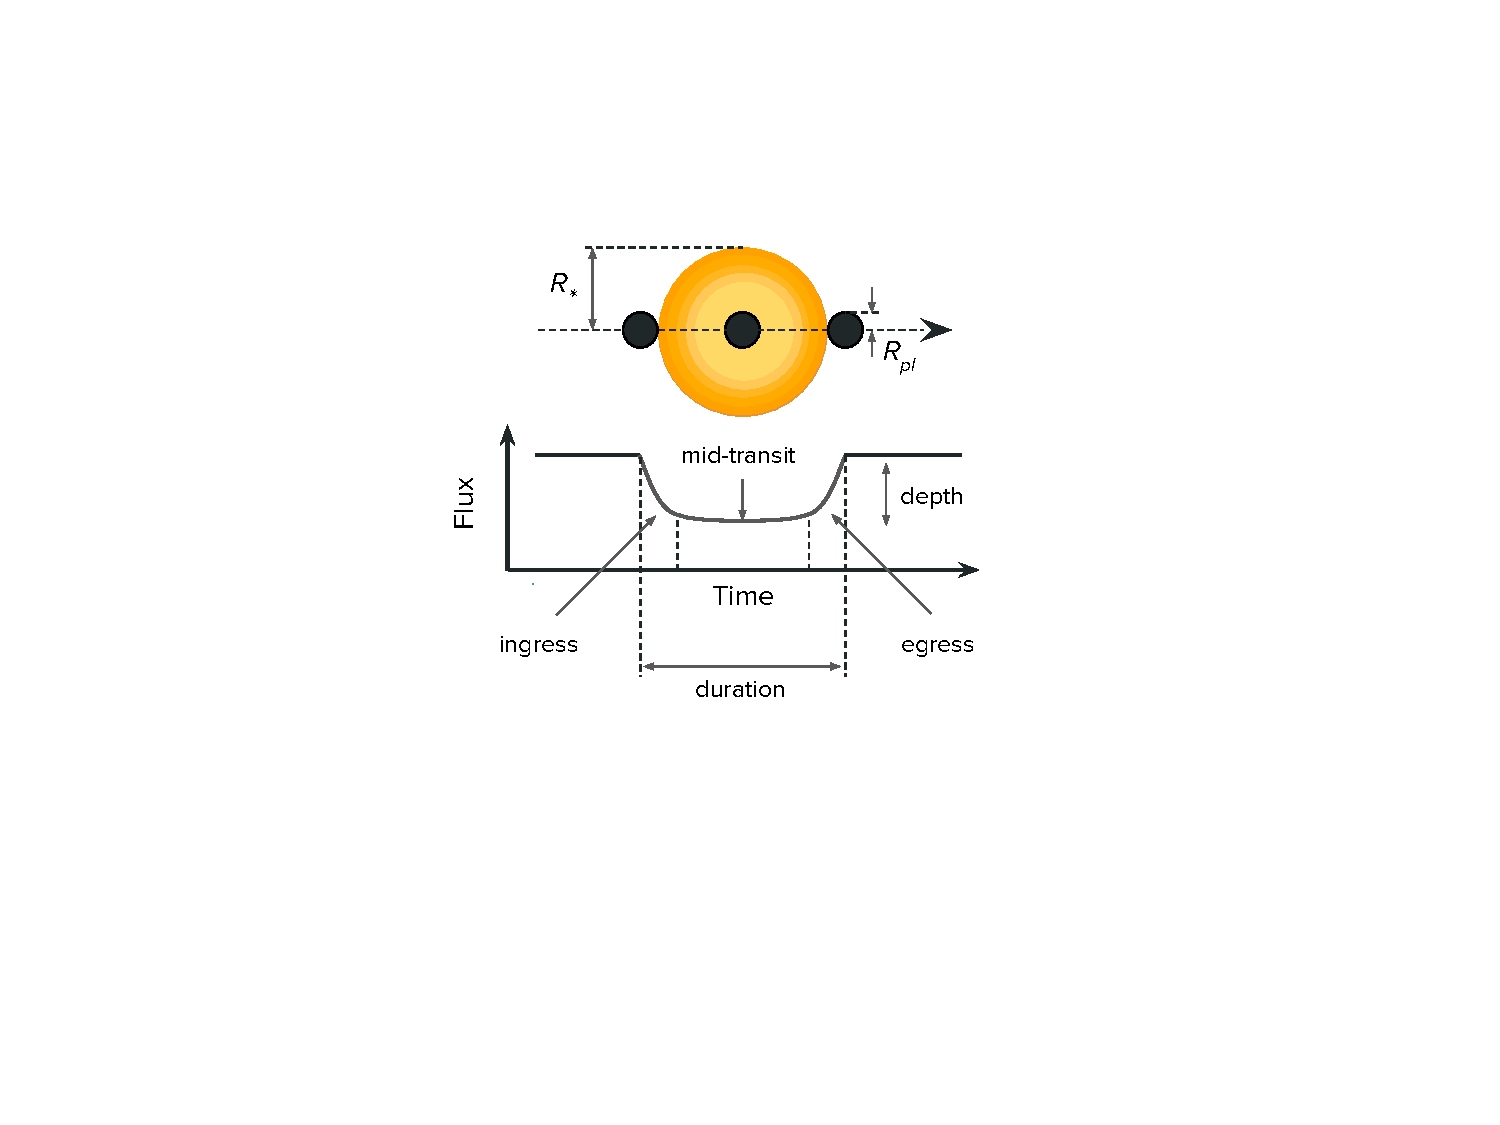
\includegraphics[width=0.4\linewidth]{Background/Figures/transit_drawing.pdf}
    \caption{\todo{caption}}
    \label{fig:transit}
\end{figure}

Figure \ref{fig:transit} illustrates the effect of a transit event on a simplified light curve of a star. The exoplanet does not contribute to the light that is observed, only to the absence of light. When the planet moves in front of the stellar disk, i.e. during ``ingress'', the observed light from the star drops. Around the mid-transit time, the amount of observed flux only changes slightly over time, depending on the distribution of light emitted from the stellar surface (see Section \ref{sec:transit_shapes}). When the planet moves away from the stellar disk, i.e. during ``egress'', the observed flux increases again to its normal level. The depth of the signal can be described by the fraction of light that is blocked by the planet, which in the case of a simplified edge-on system is $\delta = R_{pl}^2 / R_*^2$. The duration of the signal depends on the orbital period $P$ of the planet. In turn, the period of the planet depends on the semi-major axis $a$ of its orbit, according to Kepler's third law:
\begin{equation}
    \label{eq:kepler}
    P^2 = \frac{4 \pi^2}{GM}  a^3,
\end{equation}
where $G$ is the gravitational constant ($G=6.67408 \cdot 10^{-11} \text{m}^3 \text{kg}^{-1} \text{s}^{-2}$), and $M$ the star’s mass.
In case the eccentricity of the planet's orbit is 0, i.e. the orbit describes a circle, $a$ is simply the distance of the planet from its host star. For increased values for the eccentricity, the orbit becomes more elliptical. Another parameter that is relevant is the inclination $i$ of the orbit. If $i=90^\circ$, then the system is seen edge-on, meaning that the planet would transit its host star. For values $i < 90^\circ$ or $i > 90^\circ$, the planet crosses the stellar disk further away from its center, up to a point where the planet does not transit the star at all.

\begin{figure}
    \centering
    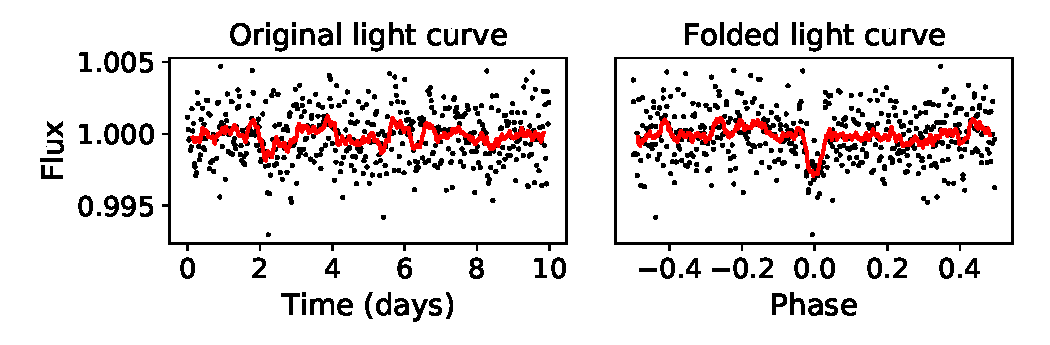
\includegraphics[width=0.6\linewidth]{Background/Figures/folding.pdf}
    \caption{\todo{caption, $P= 2.0313$d , $t_0= 0.2120$d}}
    \label{fig:folding}
\end{figure}


Figure \ref{fig:folding} shows a more realistic, but simulated light curve with five transit signals of a single planet. The light curve is dominated by white noise and the transit signals are therefore difficult to recognize. For this reason, the transit method often works better if the input light curve is ``folded'' over the period of the planet. In the resulting phase curve, the signal-to-noise ratio (SNR) of the signal is then increased compared to the individual signals in the original light curve. The problem in detection, however, is that the correct period of a planet is not known beforehand, let alone the fact that there may not be a planet in the first place.
